\begin{enumerate}[label=\thesubsection.\arabic*, ref=\thesubsection.\theenumi]
\item 
If the angle between two tangents drawn from an external point P to a circle of radius $a$ and centre O, is $60^{\circ}$, then find the length of OP.
\hfill (CBSE~2017)
\\
\solution
Let $\vec{T}_1$ and $\vec{T}_2$ be the points of contact of the tangents from $\vec{P}$. From \eqref{eq:EE26BTECH11229-tangent-equal},
\begin{align}
	\norm{\vec{P}-\vec{T}_1} = \norm{\vec{P}-\vec{T}_2}
\end{align}
Also $\norm{\vec{O}-\vec{T}_1} = \norm{\vec{O}-\vec{T}_2} = a$ and $\vec{O}\vec{P}$ is common. So the triangles $\vec{O}\vec{T}_1\vec{P}$ and $\vec{O}\vec{T}_2\vec{P}$ are congruent, and $\vec{O}\vec{P}$ bisects the angle between the tangents,
\begin{align}
	\angle \vec{O}\vec{P}\vec{T}_1 = \frac{60^{\circ}}{2} = 30^{\circ}
\end{align}
From \eqref{eq:EE26BTECH11229-tangent-perp}, the triangle $\vec{O}\vec{T}_1\vec{P}$ is right angled at $\vec{T}_1$. Using \eqref{eq:EE26BTECH11229-trig},
\begin{align}
	\sin 30^{\circ} &= \frac{a}{\norm{\vec{O}-\vec{P}}}
	\\
	\implies \norm{\vec{O}-\vec{P}} &= \frac{a}{\frac{1}{2}} = 2a
\end{align}
To verify numerically, take $a = 3$ and
\begin{align}
	\vec{O} = \myvec{0 \\ 0}, \quad \vec{P} = \myvec{6 \\ 0}
\end{align}
so that $\norm{\vec{O}-\vec{P}} = 6 = 2a$. Let $\vec{T}$ be a point of contact. From \eqref{eq:EE26BTECH11229-tangent-perp},
\begin{align}
	\brak{\vec{P}-\vec{T}}^{\top}\vec{T} = 0 \implies \vec{P}^{\top}\vec{T} = \norm{\vec{T}}^2 = a^2 = 9
\end{align}
With $\vec{T} = \myvec{x \\ y}$,
\begin{align}
	6x = 9 \implies x = \frac{3}{2}, \quad y^2 = 9 - \frac{9}{4} = \frac{27}{4} \implies y = \pm\frac{3\sqrt{3}}{2}
\end{align}
Hence, the points of contact are
\begin{align}
	\vec{T}_1 = \myvec{\frac{3}{2} \\ \frac{3\sqrt{3}}{2}}, \quad \vec{T}_2 = \myvec{\frac{3}{2} \\ -\frac{3\sqrt{3}}{2}}
\end{align}
The lengths of the tangents are
\begin{align}
	\norm{\vec{P}-\vec{T}_1} = \norm{\myvec{\frac{9}{2} \\ -\frac{3\sqrt{3}}{2}}} = \sqrt{\frac{81}{4} + \frac{27}{4}} = 3\sqrt{3} = \norm{\vec{P}-\vec{T}_2}
\end{align}
which are equal and agree with $\sqrt{\norm{\vec{P}-\vec{O}}^2 - a^2} = \sqrt{36 - 9} = 3\sqrt{3}$ from \eqref{eq:EE26BTECH11229-tangent-equal}. The angle between the tangents is the angle between $\vec{T}_1 - \vec{P}$ and $\vec{T}_2 - \vec{P}$. From \eqref{eq:EE26BTECH11229-angle-vec},
\begin{align}
	\cos\theta = \frac{\brak{\vec{T}_1-\vec{P}}^{\top}\brak{\vec{T}_2-\vec{P}}}{\norm{\vec{T}_1-\vec{P}}\norm{\vec{T}_2-\vec{P}}}
	= \frac{\frac{81}{4} - \frac{27}{4}}{27} = \frac{1}{2}
\end{align}
Hence,
\begin{align}
	\theta = 60^{\circ}
\end{align}
which verifies that $OP = 2a = 6$ for $a = 3$.
The following code generates \figref{fig:EE26BTECH11229-20}
\begin{lstlisting}[frame=single, basicstyle=\rmfamily, escapeinside={(*@}{@*)}]
(*@\makebox[\dimexpr\linewidth-2\fboxsep-2\fboxrule\relax][c]{codes/tangent\_length.py}@*)
\end{lstlisting}
\begin{figure}[H]
    \centering
    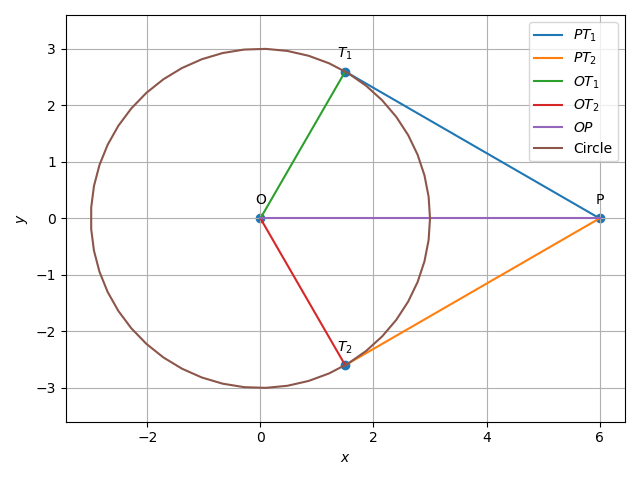
\includegraphics[width=0.75\linewidth]{figs/tangent_length.png}
    \caption{Tangents from $\vec{P}$ to the circle of radius $a = 3$}
    \label{fig:EE26BTECH11229-20}
\end{figure}

\item 
A circle touches all the four sides of a quadrilateral ABCD. Prove that 
\begin{align*}
	AB + CD = BC + DA
\end{align*}
\hfill (CBSE~2017)
\\
\solution
Let the circle touch $AB$, $BC$, $CD$ and $DA$ at $\vec{P}$, $\vec{Q}$, $\vec{R}$ and $\vec{S}$ respectively. The tangents drawn from each of $\vec{A}$, $\vec{B}$, $\vec{C}$ and $\vec{D}$ are equal, from \eqref{eq:EE26BTECH11229-tangent-equal}. Hence,
\begin{align}
	AP = AS, \quad BP = BQ, \quad CR = CQ, \quad DR = DS
	\label{eq:EE26BTECH11229-Prob_5-1}
\end{align}
Adding the above,
\begin{align}
	\brak{AP + BP} + \brak{CR + DR} = \brak{AS + DS} + \brak{BQ + CQ}
\end{align}
Since $\vec{P}$ lies on $AB$, $\vec{R}$ on $CD$, $\vec{S}$ on $DA$ and $\vec{Q}$ on $BC$, 
\begin{align}
	AP + BP = AB, \quad CR + DR = CD, \quad AS + DS = DA, \quad BQ + CQ = BC
\end{align}
Substituting in the above,
\begin{align}
	AB + CD = BC + DA
\end{align}
To verify numerically, choose
\begin{align}
	\vec{A} = \myvec{0 \\ 0}, \quad \vec{B} = \myvec{6 \\ 0}, \quad \vec{C} = \myvec{3 \\ 4}, \quad \vec{D} = \myvec{0 \\ 4}
\end{align}
The lengths of the sides are
\begin{align}
	AB = \norm{\vec{B}-\vec{A}} = 6, \quad BC = \norm{\vec{C}-\vec{B}} = 5, \quad CD = \norm{\vec{D}-\vec{C}} = 3, \quad DA = \norm{\vec{A}-\vec{D}} = 4
\end{align}
so that
\begin{align}
	AB + CD = 9 = BC + DA
\end{align}
and the given condition is satisfied. The centre $\vec{O}$ of the circle lies on the bisectors of the angles at $\vec{A}$ and $\vec{B}$. From \eqref{eq:EE26BTECH11229-angle-bisector}, the directions of these bisectors are
\begin{align}
	\vec{m}_A &= \frac{\vec{B}-\vec{A}}{\norm{\vec{B}-\vec{A}}} + \frac{\vec{D}-\vec{A}}{\norm{\vec{D}-\vec{A}}} = \myvec{1 \\ 0} + \myvec{0 \\ 1} = \myvec{1 \\ 1}
	\\
	\vec{m}_B &= \frac{\vec{A}-\vec{B}}{\norm{\vec{A}-\vec{B}}} + \frac{\vec{C}-\vec{B}}{\norm{\vec{C}-\vec{B}}} = \myvec{-1 \\ 0} + \myvec{-\frac{3}{5} \\ \frac{4}{5}} = \frac{4}{5}\myvec{-2 \\ 1}
\end{align}
Let $\vec{O} = \vec{A} + t\vec{m}_A = \vec{B} + s\myvec{-2 \\ 1}$. Then
\begin{align}
	t\myvec{1 \\ 1} + s\myvec{2 \\ -1} = \vec{B} - \vec{A} = \myvec{6 \\ 0}
\end{align}
The augmented matrix is
\begin{align}
	\myvec{1 & 2 & 6 \\ 1 & -1 & 0} \xleftrightarrow{R_2 \leftarrow R_2 - R_1} \myvec{1 & 2 & 6 \\ 0 & -3 & -6}
\end{align}
which gives $s = 2$ and $t = 2$. Therefore,
\begin{align}
	\vec{O} = \vec{A} + 2\myvec{1 \\ 1} = \myvec{2 \\ 2}
\end{align}
The radius is the distance of $\vec{O}$ from the side $AB$, which has the normal vector $\vec{n}_1 = \myvec{0 \\ 1}$. From \eqref{eq:EE26BTECH11229-dist-line},
\begin{align}
	r = \frac{\abs{\vec{n}_1^{\top}\brak{\vec{O}-\vec{A}}}}{\norm{\vec{n}_1}} = \frac{\abs{\myvec{0 & 1}\myvec{2 \\ 2}}}{1} = 2
\end{align}
To check that the circle touches the other three sides, the normal vectors of $BC$, $CD$ and $DA$ are $\vec{n}_2 = \myvec{4 \\ 3}$ (since $\vec{n}_2^{\top}\brak{\vec{C}-\vec{B}} = 0$), $\vec{n}_3 = \myvec{0 \\ 1}$ and $\vec{n}_4 = \myvec{1 \\ 0}$. Then
\begin{align}
	\frac{\abs{\vec{n}_2^{\top}\brak{\vec{O}-\vec{B}}}}{\norm{\vec{n}_2}} &= \frac{\abs{\myvec{4 & 3}\myvec{-4 \\ 2}}}{5} = 2
	\\
	\frac{\abs{\vec{n}_3^{\top}\brak{\vec{O}-\vec{C}}}}{\norm{\vec{n}_3}} &= \abs{\myvec{0 & 1}\myvec{-1 \\ -2}} = 2
	\\
	\frac{\abs{\vec{n}_4^{\top}\brak{\vec{O}-\vec{D}}}}{\norm{\vec{n}_4}} &= \abs{\myvec{1 & 0}\myvec{2 \\ -2}} = 2
\end{align}
Hence, the circle with centre $\vec{O} = \myvec{2 \\ 2}$ and radius $r = 2$ touches all four sides of the quadrilateral $ABCD$.
The following code generates \figref{fig:EE26BTECH11229-12}
\begin{lstlisting}[frame=single, basicstyle=\rmfamily, escapeinside={(*@}{@*)}]
(*@\makebox[\dimexpr\linewidth-2\fboxsep-2\fboxrule\relax][c]{codes/quad\_incircle.py}@*)
\end{lstlisting}
\begin{figure}[H]
    \centering
    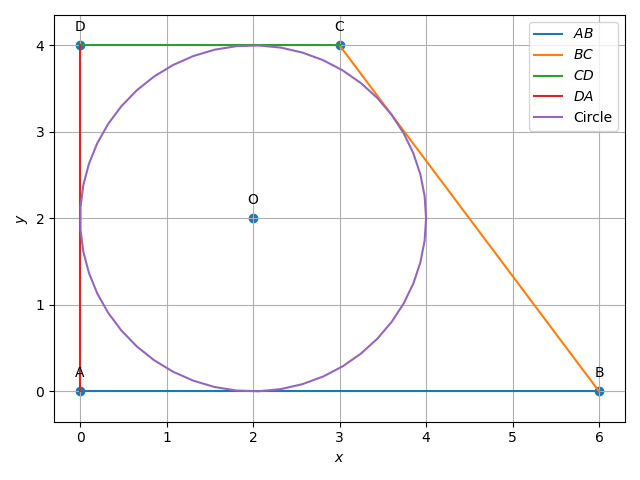
\includegraphics[width=0.75\linewidth]{figs/quad_incircle.png}
    \caption{Circle touching all four sides of the quadrilateral $ABCD$}
    \label{fig:EE26BTECH11229-12}
\end{figure}
\item 
If the distances of $\vec{P}\brak{x, y}$ from $\vec{A}\brak{5, 1}$ and $\vec{B}\brak{-1, 5}$ are equal, then prove that $3x = 2y$.
\hfill (CBSE~2017)
\\
\solution
Let
\begin{align}
	\vec{x} = \myvec{x \\ y}, \quad \vec{A} = \myvec{5 \\ 1}, \quad \vec{B} = \myvec{-1 \\ 5}
\end{align}
Then
\begin{align}
	\vec{A} - \vec{B} = \myvec{6 \\ -4}, \quad
	\norm{\vec{A}}^2 = 26, \quad \norm{\vec{B}}^2 = 26
\end{align}
Substituting in \eqref{eq:EE26BTECH11229-perp-bisector},
\begin{align}
	\myvec{6 & -4}\myvec{x \\ y} &= \frac{26 - 26}{2} = 0
	\\
	\implies 6x - 4y &= 0
	\\
	\therefore 3x &= 2y
\end{align}
The following code generates \figref{fig:EE26BTECH11229-13}
\begin{lstlisting}[frame=single, basicstyle=\rmfamily, escapeinside={(*@}{@*)}]
(*@\makebox[\dimexpr\linewidth-2\fboxsep-2\fboxrule\relax][c]{codes/perp\_bisector.py}@*)
\end{lstlisting}
\begin{figure}[H]
    \centering
    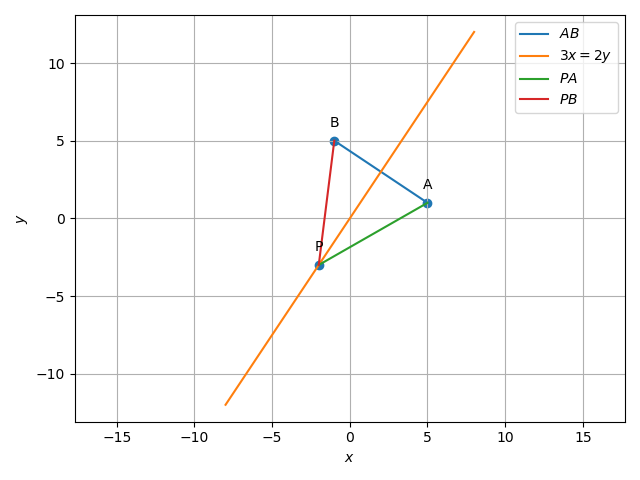
\includegraphics[width=0.75\linewidth]{figs/perp_bisector.png}
    \caption{Perpendicular bisector of $AB$}
    \label{fig:EE26BTECH11229-13}
\end{figure}
\item 
Find the value of $p$, for which one root of the quadratic equation $px^2 - 14x + 8 = 0$ is 6 times the other.
\hfill (CBSE~2017)
\\
\solution
Let the roots be $\alpha$ and $6\alpha$. From \eqref{eq:EE26BTECH11229-quad-roots},
\begin{align}
	\alpha + 6\alpha &= \frac{14}{p}
	\label{eq:EE26BTECH11229-Prob_9-1}
	\\
	\alpha \brak{6\alpha} &= \frac{8}{p}
	\label{eq:EE26BTECH11229-Prob_9-2}
\end{align}
From \eqref{eq:EE26BTECH11229-Prob_9-1}, 
\begin{align}
	\alpha = \frac{2}{p}
\end{align}
Substituting in \eqref{eq:EE26BTECH11229-Prob_9-2},
\begin{align}
	\frac{24}{p^2} &= \frac{8}{p}
	\\
	\implies p &= 3
\end{align}
For $p=3$, the roots are $4$ and $\frac{2}{3}$, and indeed $4 = 6\brak{\frac{2}{3}}$.
For $p = 3$, consider the parabola $y = 3x^2 - 14x + 8$. Its quadratic form is
\begin{align}
	\vec{x}^{\top}\vec{V}\vec{x} + 2\vec{u}^{\top}\vec{x} + f = 0
\end{align}
where
\begin{align}
	\vec{x} = \myvec{x \\ y}, \quad \vec{V} = \myvec{3 & 0 \\ 0 & 0}, \quad \vec{u} = \myvec{-7 \\ -\frac{1}{2}}, \quad f = 8
\end{align}
Since $\rank\brak{\vec{V}} = 1$, this is a parabola. The $x$-axis is the line $\vec{x} = \vec{h} + \kappa\vec{m}$ with
\begin{align}
	\vec{h} = \myvec{0 \\ 0}, \quad \vec{m} = \myvec{1 \\ 0}
\end{align}
Then
\begin{align}
	\vec{m}^{\top}\vec{V}\vec{m} = 3, \quad \vec{m}^{\top}\brak{\vec{V}\vec{h} + \vec{u}} = -7, \quad g\brak{\vec{h}} = f = 8
\end{align}
From \eqref{eq:EE26BTECH11229-conic-line}, the points of intersection of the parabola with the $x$-axis satisfy
\begin{align}
	3\kappa^2 - 14\kappa + 8 = 0
\end{align}
which is the same equation as the given quadratic equation for $p = 3$. From \eqref{eq:EE26BTECH11229-quad-formula},
\begin{align}
	\kappa = \frac{14 \pm \sqrt{196 - 96}}{6} = \frac{14 \pm 10}{6} = 4 \text{ or } \frac{2}{3}
\end{align}
Therefore, the parabola meets the $x$-axis at
\begin{align}
	\vec{x} = \kappa\vec{m} = \myvec{4 \\ 0} \text{ and } \myvec{\frac{2}{3} \\ 0}
\end{align}
so the roots of the quadratic equation are the intersections of the parabola with the $x$-axis.
The following code generates \figref{fig:EE26BTECH11229-16}
\begin{lstlisting}[frame=single, basicstyle=\rmfamily, escapeinside={(*@}{@*)}]
(*@\makebox[\dimexpr\linewidth-2\fboxsep-2\fboxrule\relax][c]{codes/root\_ratio.py}@*)
\end{lstlisting}
\begin{figure}[H]
    \centering
    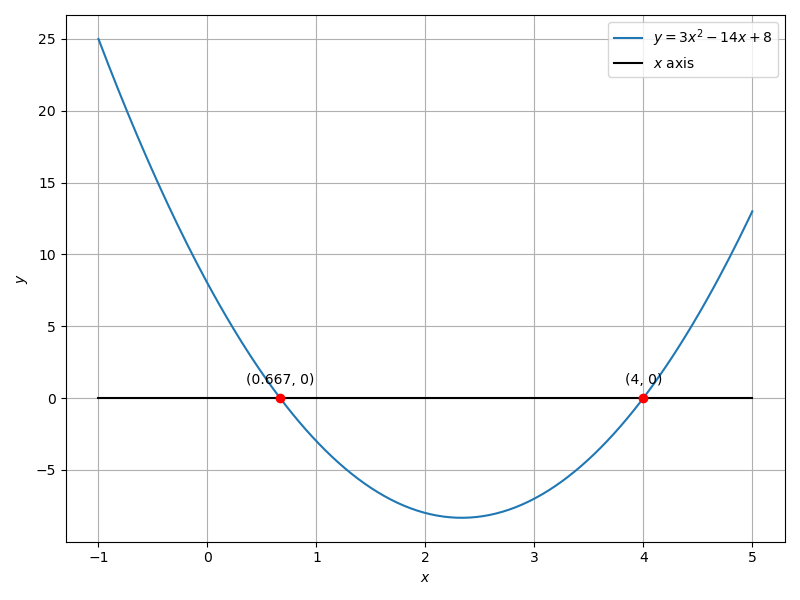
\includegraphics[width=0.75\linewidth]{figs/root_ratio.png}
    \caption{Parabola $y = 3x^2 - 14x + 8$ meeting the $x$-axis at $x = \frac{2}{3}$ and $x = 4$}
    \label{fig:EE26BTECH11229-16}
\end{figure}

\item 
For what value of $n$, are the $n^{\text{th}}$ terms of two A.Ps $63, 65, 67, \ldots$ and $3, 10, 17, \ldots$ equal ?
\hfill (CBSE~2017)
\\
\solution
Let the index start from $0$, so that $x\brak{n}$ is the $\brak{n+1}^{\text{th}}$ term. From \eqref{eq:EE26BTECH11229-ap-step}, with $a = 63$, $d = 2$ for the first A.P. and $a = 3$, $d = 7$ for the second A.P.,
\begin{align}
	x_1\brak{n} = \brak{63 + 2n}u\brak{n}, \quad x_2\brak{n} = \brak{3 + 7n}u\brak{n}
\end{align}
The two sequences intersect when $x_1\brak{n} = x_2\brak{n}$ for $n \ge 0$,
\begin{align}
	63 + 2n &= 3 + 7n
	\\
	\implies 5n &= 60
	\\
	\therefore n &= 12
\end{align}
Hence, the stems of the two sequences coincide at $n = 12$, where
\begin{align}
	x_1\brak{12} = 63 + 24 = 87, \quad x_2\brak{12} = 3 + 84 = 87
\end{align}
Since $x\brak{n}$ is the $\brak{n+1}^{\text{th}}$ term, the $13^{\text{th}}$ terms of the two A.Ps are equal.
The following code verifies the solution
\begin{lstlisting}[frame=single, basicstyle=\rmfamily, escapeinside={(*@}{@*)}]
(*@\makebox[\dimexpr\linewidth-2\fboxsep-2\fboxrule\relax][c]{codes/ap\_equal.c}@*)
\end{lstlisting}
The following code generates \figref{fig:EE26BTECH11229-17}
\begin{lstlisting}[frame=single, basicstyle=\rmfamily, escapeinside={(*@}{@*)}]
(*@\makebox[\dimexpr\linewidth-2\fboxsep-2\fboxrule\relax][c]{codes/ap\_equal.py}@*)
\end{lstlisting}
\begin{figure}[H]
    \centering
    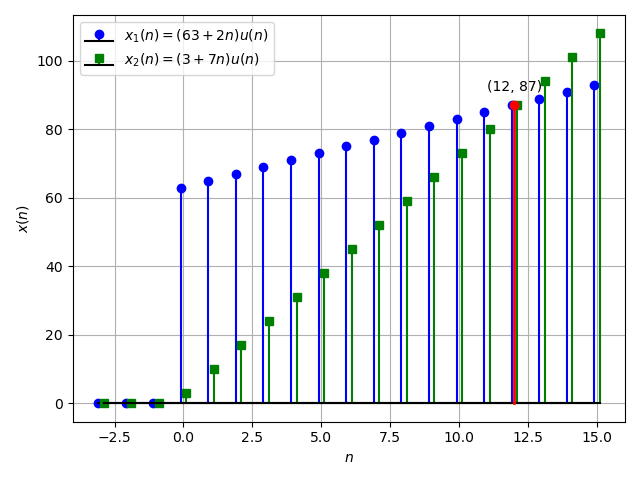
\includegraphics[width=0.75\linewidth]{figs/ap_equal.png}
    \caption{Stem plot of the two A.Ps, intersecting at $n = 12$}
    \label{fig:EE26BTECH11229-17}
\end{figure}
\item 
On a straight line passing through the foot of a tower, two points C and D are at distances of 4 m and 16 m from the foot respectively. If the angles of elevation from C and D of the top of the tower are complementary, then find the height of the tower.
\hfill (CBSE~2017)
\\
\solution
Let the foot of the tower be the origin, with the tower along the $y$-axis and $C$, $D$ on the positive $x$-axis. Let $h$ be the height of the tower. Then
\begin{align}
	\vec{O} = \myvec{0 \\ 0}, \quad \vec{C} = \myvec{4 \\ 0}, \quad \vec{D} = \myvec{16 \\ 0}, \quad \vec{T} = \myvec{0 \\ h}
\end{align}
where $\vec{T}$ is the top of the tower. Let $\theta$ be the angle of elevation from $\vec{C}$, that is, the angle between $\vec{T}-\vec{C}$ and $\vec{O}-\vec{C}$. The angle of elevation from $\vec{D}$ is then $90^{\circ}-\theta$. The vectors are
\begin{align}
	\vec{T}-\vec{C} = \myvec{-4 \\ h}, \quad \vec{O}-\vec{C} = \myvec{-4 \\ 0}, \quad
	\vec{T}-\vec{D} = \myvec{-16 \\ h}, \quad \vec{O}-\vec{D} = \myvec{-16 \\ 0}
\end{align}
From \eqref{eq:EE26BTECH11229-angle-vec},
\begin{align}
	\cos\theta &= \frac{\brak{\vec{T}-\vec{C}}^{\top}\brak{\vec{O}-\vec{C}}}{\norm{\vec{T}-\vec{C}}\norm{\vec{O}-\vec{C}}} = \frac{16}{4\sqrt{16+h^2}} = \frac{4}{\sqrt{16+h^2}}
	\\
	\cos\brak{90^{\circ}-\theta} &= \frac{\brak{\vec{T}-\vec{D}}^{\top}\brak{\vec{O}-\vec{D}}}{\norm{\vec{T}-\vec{D}}\norm{\vec{O}-\vec{D}}} = \frac{16}{\sqrt{256+h^2}}
\end{align}
Since $\cos\brak{90^{\circ}-\theta} = \sin\theta$, we have $\cos^2\theta + \cos^2\brak{90^{\circ}-\theta} = 1$,
\begin{align}
	\frac{16}{16+h^2} + \frac{256}{256+h^2} &= 1
	\\
	\implies 16\brak{256+h^2} + 256\brak{16+h^2} &= \brak{16+h^2}\brak{256+h^2}
	\\
	\implies h^4 &= 4096
	\\
	\therefore h &= 8 \text{ m}
\end{align}
The following code generates \figref{fig:EE26BTECH11229-5}
\begin{lstlisting}[frame=single, basicstyle=\rmfamily, escapeinside={(*@}{@*)}]
(*@\makebox[\dimexpr\linewidth-2\fboxsep-2\fboxrule\relax][c]{codes/trig\_height.py}@*)
\end{lstlisting}
\begin{figure}[H]
    \centering
    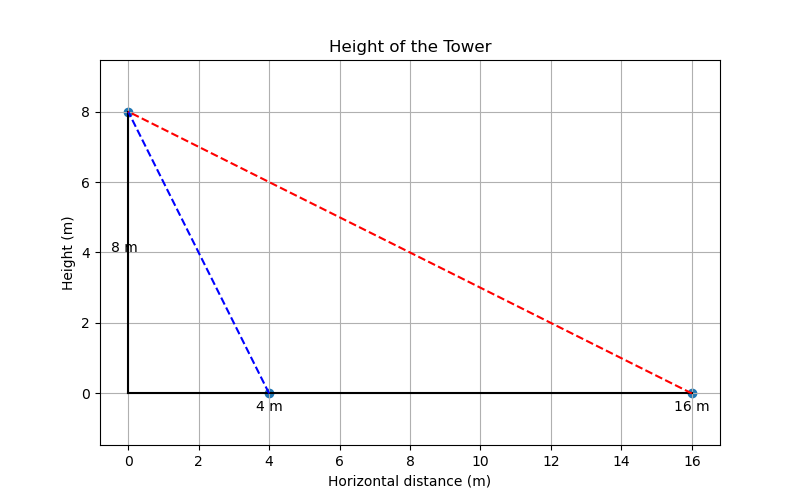
\includegraphics[width=0.75\linewidth]{figs/trig_height.png}
    \caption{Tower and the angles of elevation}
    \label{fig:EE26BTECH11229-5}
\end{figure}

\item 
In what ratio does the point $\brak{\frac{24}{11}, y}$ divide the line segment joining the points $\vec{P}\brak{2, -2}$ and $\vec{Q}\brak{3, 7}$ ? Also find the value of $y$.
\hfill (CBSE~2017)
\\
\solution
Let $\vec{R} = \myvec{\frac{24}{11} \\ y}$. Since $\vec{R}$ lies on the line segment joining $\vec{P}$ and $\vec{Q}$, the points $\vec{P}$, $\vec{Q}$ and $\vec{R}$ are collinear. Then
\begin{align}
	\vec{Q} - \vec{P} = \myvec{1 \\ 9}, \quad \vec{R} - \vec{P} = \myvec{\frac{2}{11} \\ y+2}
\end{align}
From \eqref{eq:EE26BTECH11229-collinear},
\begin{align}
	\rank\myvec{\vec{Q}-\vec{P} & \vec{R}-\vec{P}} = \rank\myvec{1 & \frac{2}{11} \\ 9 & y+2} = 1
\end{align}
Performing the row operation $R_2 \leftarrow R_2 - 9R_1$,
\begin{align}
	\myvec{1 & \frac{2}{11} \\ 9 & y+2} \xleftrightarrow{R_2 \leftarrow R_2 - 9R_1} \myvec{1 & \frac{2}{11} \\ 0 & y + 2 - \frac{18}{11}}
\end{align}
For the rank to be $1$, the second row must vanish,
\begin{align}
	y + 2 - \frac{18}{11} = 0 \implies y = -\frac{4}{11}
\end{align}
The second column is also $\frac{2}{11}$ times the first column, so
\begin{align}
	\vec{R} - \vec{P} = \frac{2}{11}\brak{\vec{Q} - \vec{P}}
\end{align}
From \eqref{eq:EE26BTECH11229-ratio-collinear} with $\lambda = \frac{2}{11}$,
\begin{align}
	\vec{P}\vec{R} : \vec{R}\vec{Q} = \lambda : \brak{1-\lambda} = \frac{2}{11} : \frac{9}{11} = 2 : 9
\end{align}
Thus, the ratio is $2:9$ and $y = -\frac{4}{11}$.
The following code verifies the solution
\begin{lstlisting}[frame=single, basicstyle=\rmfamily, escapeinside={(*@}{@*)}]
(*@\makebox[\dimexpr\linewidth-2\fboxsep-2\fboxrule\relax][c]{codes/section.c}@*)
\end{lstlisting}
\item 
How many terms of an A.P. $9, 17, 25, \ldots$ must be taken to give a sum of 636 ?
\hfill (CBSE~2017)
\\
\solution
Let $x\brak{n}$ be the $\brak{n+1}^{\text{th}}$ term of the A.P. $9, 17, 25, \ldots$, where $n = 0, 1, 2, \ldots$ Then
\begin{align}
	x\brak{n} = \brak{9 + 8n}u\brak{n}
\end{align}
The sum of the first $n+1$ terms is
\begin{align}
	y\brak{n} = \sum_{k=0}^{n} x\brak{k} = x\brak{n} * u\brak{n}
\end{align}
From \eqref{eq:EE26BTECH11229-z-prop}, for $\abs{z} > 1$,
\begin{align}
	Y\brak{z} = \frac{X\brak{z}}{1 - z^{-1}}
\end{align}
Using \eqref{eq:EE26BTECH11229-z-pairs},
\begin{align}
	X\brak{z} &= \frac{9}{1 - z^{-1}} + \frac{8z^{-1}}{\brak{1 - z^{-1}}^2} = \frac{9 - z^{-1}}{\brak{1 - z^{-1}}^2}
	\\
	\implies Y\brak{z} &= \frac{9 - z^{-1}}{\brak{1 - z^{-1}}^3} = \frac{9}{\brak{1 - z^{-1}}^3} - \frac{z^{-1}}{\brak{1 - z^{-1}}^3}
\end{align}
Taking the inverse Z-transform using \eqref{eq:EE26BTECH11229-z-pairs} and \eqref{eq:EE26BTECH11229-z-prop},
\begin{align}
	y\brak{n} &= 9\cdot\frac{\brak{n+1}\brak{n+2}}{2}u\brak{n} - \frac{n\brak{n+1}}{2}u\brak{n-1}
\end{align}
The second term is zero at $n = 0$, so $u\brak{n-1}$ can be replaced by $u\brak{n}$,
\begin{align}
	y\brak{n} = \frac{\brak{n+1}\brak{9n + 18 - n}}{2}u\brak{n} = \brak{n+1}\brak{4n+9}u\brak{n}
\end{align}
Equating the sum to $636$,
\begin{align}
	\brak{n+1}\brak{4n+9} &= 636
	\\
	\implies 4n^2 + 13n - 627 &= 0
\end{align}
From \eqref{eq:EE26BTECH11229-quad-formula},
\begin{align}
	n = \frac{-13 \pm \sqrt{169 + 10032}}{8} = \frac{-13 \pm 101}{8}
\end{align}
Since $n \ge 0$,
\begin{align}
	n = 11
\end{align}
Hence, the number of terms is $n + 1 = 12$.
The following code verifies the solution
\begin{lstlisting}[frame=single, basicstyle=\rmfamily, escapeinside={(*@}{@*)}]
(*@\makebox[\dimexpr\linewidth-2\fboxsep-2\fboxrule\relax][c]{codes/ap\_sum.c}@*)
\end{lstlisting}
\item 
If the points $\vec{A}\brak{k+1, 2k}$, $\vec{B}\brak{3k, 2k+3}$ and $\vec{C}\brak{5k-1, 5k}$ are collinear, then find the value of $k$.
\hfill (CBSE~2017)
\\
\solution
Let
\begin{align}
	\vec{B} - \vec{A} = \myvec{2k-1 \\ 3}, \quad \vec{C} - \vec{A} = \myvec{4k-2 \\ 3k}
\end{align}
From \eqref{eq:EE26BTECH11229-collinear}, the points are collinear if and only if
\begin{align}
	\rank\myvec{\vec{B}-\vec{A} & \vec{C}-\vec{A}} = \rank\myvec{2k-1 & 4k-2 \\ 3 & 3k} = 1
\end{align}
Performing the row operations $R_1 \leftrightarrow R_2$ and $R_1 \leftarrow \frac{R_1}{3}$,
\begin{align}
	\myvec{2k-1 & 4k-2 \\ 3 & 3k} \xleftrightarrow[R_1 \leftarrow \frac{R_1}{3}]{R_1 \leftrightarrow R_2} \myvec{1 & k \\ 2k-1 & 4k-2}
\end{align}
Performing the row operation $R_2 \leftarrow R_2 - \brak{2k-1}R_1$,
\begin{align}
	\myvec{1 & k \\ 2k-1 & 4k-2} \xleftrightarrow{R_2 \leftarrow R_2 - \brak{2k-1}R_1} \myvec{1 & k \\ 0 & -2k^2 + 5k - 2}
\end{align}
The first row is nonzero, so for the rank to be $1$, the second row must vanish,
\begin{align}
	-2k^2 + 5k - 2 &= 0
	\\
	\implies 2k^2 - 5k + 2 &= 0
	\\
	\implies \brak{2k-1}\brak{k-2} &= 0
\end{align}
Hence,
\begin{align}
	k = \frac{1}{2} \quad \text{or} \quad k = 2
\end{align}
\item 
Two different dice are thrown together. Find the probability that the numbers obtained have
\begin{enumerate}
	\item even sum, and
	\item even product.
\end{enumerate}
\hfill (CBSE~2017)
\\
\solution
Let $X_1$ and $X_2$ represent the scores on the two dice, and let $X = X_1 + X_2$ denote their sum.
\begin{enumerate}
\item From the triangular PMF in \eqref{eq:EE26BTECH11229-dice-pmf}, the sum is even for $n \in \{2, 4, 6, 8, 10, 12\}$. Hence,
\begin{align}
	\pr{X \text{ is even}} &= \sum_{n \in \{2, 4, 6, 8, 10, 12\}} p_X\brak{n}
	\\
	&= \frac{1 + 3 + 5 + 5 + 3 + 1}{36} = \frac{1}{2}
\end{align}
\item The product $X_1 X_2$ is odd if and only if both $X_1$ and $X_2$ are odd. From \eqref{eq:EE26BTECH11229-dice-uniform},
\begin{align}
	\pr{X_1 \text{ is odd}} = p_{X_1}\brak{1} + p_{X_1}\brak{3} + p_{X_1}\brak{5} = \frac{3}{6} = \frac{1}{2}
\end{align}
and similarly $\pr{X_2 \text{ is odd}} = \frac{1}{2}$. Since $X_1$ and $X_2$ are independent,
\begin{align}
	\pr{X_1 X_2 \text{ is odd}} = \frac{1}{2} \cdot \frac{1}{2} = \frac{1}{4}
\end{align}
Using the complement in \eqref{eq:EE26BTECH11229-prob-def},
\begin{align}
	\pr{X_1 X_2 \text{ is even}} = 1 - \frac{1}{4} = \frac{3}{4}
\end{align}
\end{enumerate}
\item 
In the given figure, $XY$ and $X^{\prime}Y^{\prime}$ are two parallel tangents to a circle with centre O and another tangent $AB$ with point of contact $C$, is intersecting $XY$ at $A$ and $X^{\prime}Y^{\prime}$ at $B$. Prove that $\angle AOB = 90^{\circ}$.
\hfill (CBSE~2017)
\begin{figure}[H]
	\centering
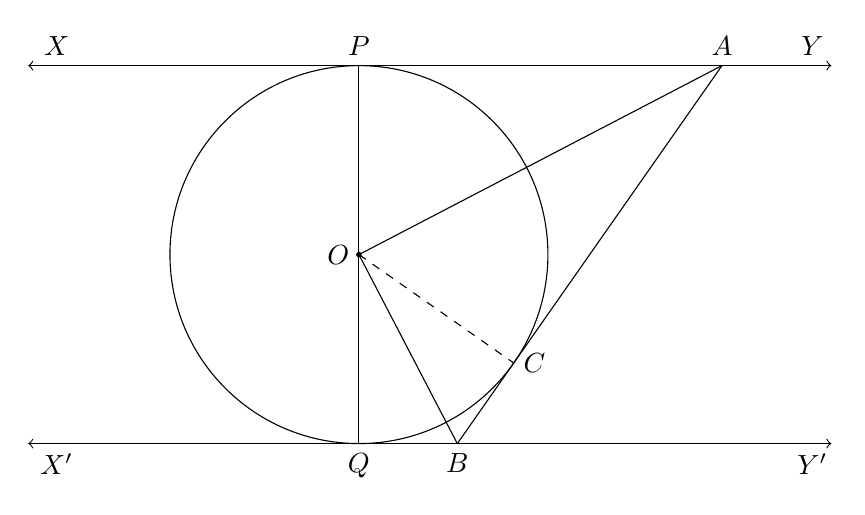
\begin{tikzpicture}[scale=1.2]
\coordinate (O) at (0,0);
\coordinate (P) at (0,2);
\coordinate (Q) at (0,-2);
\coordinate (C) at (-35:2);
\coordinate (A) at ({(2-2*sin(-35))/cos(-35)},2);
\coordinate (B) at ({(2+2*sin(-35))/cos(-35)},-2);
% circle and parallel tangents
\draw (O) circle (2);
\draw[<->] (-3.5,2) -- (5,2);
\draw[<->] (-3.5,-2) -- (5,-2);
% diameter PQ and tangent AB
\draw (P) -- (Q);
\draw (A) -- (B);
\draw (O) -- (A);
\draw (O) -- (B);
\draw[dashed] (O) -- (C);
\fill (O) circle (0.03);
% labels
\node[above] at (-3.2,2) {$X$};
\node[above] at (4.8,2) {$Y$};
\node[above] at (P) {$P$};
\node[above] at (A) {$A$};
\node[below] at (-3.2,-2) {$X^{\prime}$};
\node[below] at (4.8,-2) {$Y^{\prime}$};
\node[below] at (Q) {$Q$};
\node[below] at (B) {$B$};
\node[left] at (O) {$O$};
\node[right] at (C) {$C$};
\end{tikzpicture}
\caption{}
    \label{fig:EE26BTECH11229-3}
\end{figure}
\solution
In \figref{fig:EE26BTECH11229-3}, let $r$ be the radius of the circle, and let $P$, $Q$ and $C$ be the points of contact of $XY$, $X^{\prime}Y^{\prime}$ and $AB$. Take $\vec{O}$ as the origin with $XY \parallel X^{\prime}Y^{\prime}$ along the $x$-direction. Since the tangents at $P$ and $Q$ are parallel, from \eqref{eq:EE26BTECH11229-tangent-perp}, $P$, $O$ and $Q$ are collinear,
\begin{align}
	\vec{O} = \myvec{0 \\ 0}, \quad \vec{P} = \myvec{0 \\ r}, \quad \vec{Q} = \myvec{0 \\ -r}, \quad \vec{C} = \myvec{c_1 \\ c_2}, \quad c_1^2 + c_2^2 = r^2
\end{align}
The points $\vec{A}$ and $\vec{B}$ lie on the tangents $XY$ and $X^{\prime}Y^{\prime}$ respectively, so
\begin{align}
	\vec{A} = \myvec{a \\ r}, \quad \vec{B} = \myvec{b \\ -r}
\end{align}
$AB$ touches the circle at $\vec{C}$ and $\vec{A}$, $\vec{B}$ lie on this tangent. From \eqref{eq:EE26BTECH11229-tangent-perp} with $\vec{O}$ as the origin,
\begin{align}
	\brak{\vec{A}-\vec{C}}^{\top}\vec{C} = 0 &\implies \vec{A}^{\top}\vec{C} = \norm{\vec{C}}^2 = r^2
	\\
	\brak{\vec{B}-\vec{C}}^{\top}\vec{C} = 0 &\implies \vec{B}^{\top}\vec{C} = r^2
\end{align}
Substituting the coordinates,
\begin{align}
	a c_1 + r c_2 &= r^2 \implies a c_1 = r\brak{r - c_2}
	\\
	b c_1 - r c_2 &= r^2 \implies b c_1 = r\brak{r + c_2}
\end{align}
Multiplying the two equations,
\begin{align}
	ab\,c_1^2 = r^2\brak{r^2 - c_2^2} = r^2 c_1^2
\end{align}
Since $c_1 \neq 0$ (otherwise $AB$ would coincide with $XY$ or $X^{\prime}Y^{\prime}$),
\begin{align}
	ab = r^2
\end{align}
From \eqref{eq:EE26BTECH11229-angle-vec},
\begin{align}
	\cos\angle AOB = \frac{\vec{A}^{\top}\vec{B}}{\norm{\vec{A}}\norm{\vec{B}}}
	= \frac{ab - r^2}{\norm{\vec{A}}\norm{\vec{B}}} = 0
\end{align}
Hence,
\begin{align}
	\angle AOB = 90^{\circ}
\end{align}
To verify numerically, take a circle with centre $\vec{O}$ and radius $r = 10$, and the point of contact $\vec{C}$ of $AB$,
\begin{align}
	\vec{O} = \myvec{0 \\ 0}, \quad \vec{P} = \myvec{0 \\ 10}, \quad \vec{Q} = \myvec{0 \\ -10}, \quad \vec{C} = \myvec{8 \\ -6}
\end{align}
Here $\norm{\vec{C}}^2 = 64 + 36 = 100 = r^2$, so $\vec{C}$ lies on the circle. The points $\vec{A}$ and $\vec{B}$ lie on the tangents $y = 10$ and $y = -10$ respectively, so let
\begin{align}
	\vec{A} = \myvec{a \\ 10}, \quad \vec{B} = \myvec{b \\ -10}
\end{align}
From \eqref{eq:EE26BTECH11229-tangent-perp}, $\vec{A}^{\top}\vec{C} = \vec{B}^{\top}\vec{C} = r^2 = 100$,
\begin{align}
	8a - 60 &= 100 \implies a = 20
	\\
	8b + 60 &= 100 \implies b = 5
\end{align}
Hence,
\begin{align}
	\vec{A} = \myvec{20 \\ 10}, \quad \vec{B} = \myvec{5 \\ -10}
\end{align}
Then $ab = 100 = r^2$, and the tangent $AB$ is perpendicular to the radius at $\vec{C}$,
\begin{align}
	\brak{\vec{A}-\vec{C}}^{\top}\vec{C} &= \myvec{12 & 16}\myvec{8 \\ -6} = 0
	\\
	\brak{\vec{B}-\vec{C}}^{\top}\vec{C} &= \myvec{-3 & -4}\myvec{8 \\ -6} = 0
\end{align}
The tangent lengths from $\vec{A}$ and $\vec{B}$ are equal, from \eqref{eq:EE26BTECH11229-tangent-equal},
\begin{align}
	\norm{\vec{A}-\vec{P}} = \norm{\myvec{20 \\ 0}} = 20 = \norm{\myvec{12 \\ 16}} = \norm{\vec{A}-\vec{C}}
	\\
	\norm{\vec{B}-\vec{Q}} = \norm{\myvec{5 \\ 0}} = 5 = \norm{\myvec{-3 \\ -4}} = \norm{\vec{B}-\vec{C}}
\end{align}
Finally, from \eqref{eq:EE26BTECH11229-angle-vec},
\begin{align}
	\cos\angle AOB = \frac{\vec{A}^{\top}\vec{B}}{\norm{\vec{A}}\norm{\vec{B}}}
	= \frac{100 - 100}{\sqrt{500}\sqrt{125}} = 0
	\\
	\implies \angle AOB = 90^{\circ}
\end{align}
which verifies the result.
The following code generates \figref{fig:EE26BTECH11229-18}
\begin{lstlisting}[frame=single, basicstyle=\rmfamily, escapeinside={(*@}{@*)}]
(*@\makebox[\dimexpr\linewidth-2\fboxsep-2\fboxrule\relax][c]{codes/tangent\_angle.py}@*)
\end{lstlisting}
\begin{figure}[H]
    \centering
    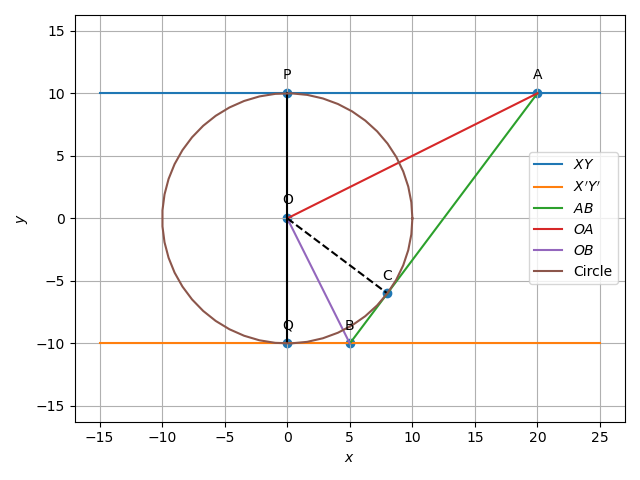
\includegraphics[width=0.75\linewidth]{figs/tangent_angle.png}
    \caption{Tangents from $\vec{h}$ to the circle, with the points of contact $\vec{T}_1$ and $\vec{T}_2$}
    \label{fig:EE26BTECH11229-18}
\end{figure}
\item 
Prove that the lengths of two tangents drawn from an external point to a circle are equal.
\hfill (CBSE~2017)
\\
\solution
Let $\vec{P}$ be an external point of a circle with centre $\vec{O}$ and radius $a$. Let the tangents from $\vec{P}$ touch the circle at $\vec{T}_1$ and $\vec{T}_2$. From \eqref{eq:EE26BTECH11229-tangent-perp}, the triangles $\vec{O}\vec{T}_1\vec{P}$ and $\vec{O}\vec{T}_2\vec{P}$ are right angled at $\vec{T}_1$ and $\vec{T}_2$. By Pythagoras' theorem,
\begin{align}
	\norm{\vec{P}-\vec{T}_1}^2 &= \norm{\vec{P}-\vec{O}}^2 - \norm{\vec{T}_1-\vec{O}}^2 = \norm{\vec{P}-\vec{O}}^2 - a^2
	\\
	\norm{\vec{P}-\vec{T}_2}^2 &= \norm{\vec{P}-\vec{O}}^2 - \norm{\vec{T}_2-\vec{O}}^2 = \norm{\vec{P}-\vec{O}}^2 - a^2
\end{align}
Therefore,
\begin{align}
	\norm{\vec{P}-\vec{T}_1} = \norm{\vec{P}-\vec{T}_2}
\end{align}
To verify numerically, take a circle with centre $\vec{O} = \myvec{0 \\ 0}$ and radius $r = 5$, and the external point $\vec{h} = \myvec{5 \\ 10}$. From \eqref{eq:EE26BTECH11229-circle},
\begin{align}
	\vec{V} = \vec{I}, \quad \vec{u} = -\vec{O} = \myvec{0 \\ 0}, \quad f = \norm{\vec{O}}^2 - r^2 = -25
\end{align}
and
\begin{align}
	g\brak{\vec{h}} = \norm{\vec{h}}^2 + 2\vec{u}^{\top}\vec{h} + f = 125 - 25 = 100 > 0
\end{align}
so $\vec{h}$ is an external point. From \eqref{eq:EE26BTECH11229-sigma},
\begin{align}
	\vec{\Sigma} = \myvec{5 \\ 10}\myvec{5 & 10} - 100\vec{I} = \myvec{-75 & 50 \\ 50 & 0}
\end{align}
The eigenvalues are the roots of
\begin{align}
	\mydet{\lambda\vec{I} - \vec{\Sigma}} \Rightarrow \lambda^2 + 75\lambda - 2500 = \brak{\lambda - 25}\brak{\lambda + 100} = 0
\end{align}
so $\lambda_1 = 25$ and $\lambda_2 = -100$. For $\lambda_1 = 25$, using row reduction,
\begin{align}
	\vec{\Sigma} - 25\vec{I} = \myvec{-100 & 50 \\ 50 & -25} \xleftrightarrow[R_2 \leftarrow R_2 - 50R_1]{R_1 \leftarrow -\frac{R_1}{100}} \myvec{1 & -\frac{1}{2} \\ 0 & 0} \implies \vec{p}_1 = \myvec{1 \\ 2}
\end{align}
For $\lambda_2 = -100$,
\begin{align}
	\vec{\Sigma} + 100\vec{I} = \myvec{25 & 50 \\ 50 & 100} \xleftrightarrow[R_2 \leftarrow R_2 - 50R_1]{R_1 \leftarrow \frac{R_1}{25}} \myvec{1 & 2 \\ 0 & 0} \implies \vec{p}_2 = \myvec{2 \\ -1}
\end{align}
Hence,
\begin{align}
	\vec{D} = \myvec{25 & 0 \\ 0 & -100}, \quad \vec{P} = \frac{1}{\sqrt{5}}\myvec{1 & 2 \\ 2 & -1}
\end{align}
Here $\vec{P}^{\top}\vec{P} = \vec{I}$, so $\vec{P}^{\top} = \vec{P}^{-1}$, and one can verify that $\vec{P}^{\top}\vec{\Sigma}\vec{P} = \vec{D}$. From \eqref{eq:EE26BTECH11229-tangent-dir}, the direction vectors of the tangents are
\begin{align}
	\vec{m} = \vec{P}\myvec{\sqrt{100} \\ \pm\sqrt{25}} = \frac{1}{\sqrt{5}}\myvec{1 & 2 \\ 2 & -1}\myvec{10 \\ \pm 5}
	= \frac{1}{\sqrt{5}}\myvec{20 \\ 15} \text{ or } \frac{1}{\sqrt{5}}\myvec{0 \\ 25}
\end{align}
Only the direction of $\vec{m}$ matters, since $\mu\vec{m}$ does not change on scaling $\vec{m}$. So take
\begin{align}
	\vec{m}_1 = \myvec{4 \\ 3}, \quad \vec{m}_2 = \myvec{0 \\ 1}
\end{align}
From \eqref{eq:EE26BTECH11229-contact}, the points of contact $\vec{T}_i = \vec{h} + \mu_i\vec{m}_i$ are given by
\begin{align}
	\mu_1 &= -\frac{\vec{m}_1^{\top}\brak{\vec{h}+\vec{u}}}{\vec{m}_1^{\top}\vec{m}_1} = -\frac{50}{25} = -2, \quad
	\vec{T}_1 = \myvec{5 \\ 10} - 2\myvec{4 \\ 3} = \myvec{-3 \\ 4}
	\\
	\mu_2 &= -\frac{\vec{m}_2^{\top}\brak{\vec{h}+\vec{u}}}{\vec{m}_2^{\top}\vec{m}_2} = -\frac{10}{1} = -10, \quad
	\vec{T}_2 = \myvec{5 \\ 10} - 10\myvec{0 \\ 1} = \myvec{5 \\ 0}
\end{align}
Both points lie on the circle, since $\norm{\vec{T}_1}^2 = 9 + 16 = 25$ and $\norm{\vec{T}_2}^2 = 25$. Also, from \eqref{eq:EE26BTECH11229-tangent-perp},
\begin{align}
	\brak{\vec{h}-\vec{T}_1}^{\top}\brak{\vec{T}_1-\vec{O}} &= \myvec{8 & 6}\myvec{-3 \\ 4} = 0
	\\
	\brak{\vec{h}-\vec{T}_2}^{\top}\brak{\vec{T}_2-\vec{O}} &= \myvec{0 & 10}\myvec{5 \\ 0} = 0
\end{align}
so the tangents are perpendicular to the radii. The lengths of the tangents are
\begin{align}
	\norm{\vec{h}-\vec{T}_1} &= \norm{\myvec{8 \\ 6}} = 10
	\\
	\norm{\vec{h}-\vec{T}_2} &= \norm{\myvec{0 \\ 10}} = 10
\end{align}
which are equal and agree with $\sqrt{\norm{\vec{h}-\vec{O}}^2 - r^2} = \sqrt{125 - 25} = 10$ from \eqref{eq:EE26BTECH11229-tangent-equal}.
The following code generates \figref{fig:EE26BTECH11229-21}
\begin{lstlisting}[frame=single, basicstyle=\rmfamily, escapeinside={(*@}{@*)}]
(*@\makebox[\dimexpr\linewidth-2\fboxsep-2\fboxrule\relax][c]{codes/tangent\_equal.py}@*)
\end{lstlisting}
\begin{figure}[H]
    \centering
    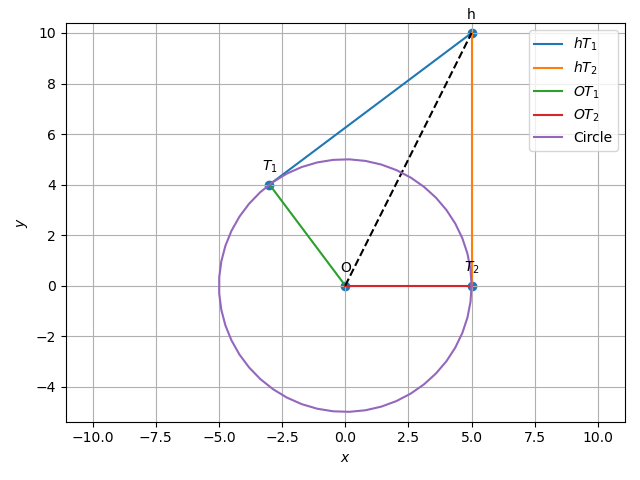
\includegraphics[width=0.75\linewidth]{figs/tangent_equal.png}
    \caption{Equal tangent lengths $\norm{\vec{P}-\vec{T}_1} = \norm{\vec{P}-\vec{T}_2}$}
    \label{fig:EE26BTECH11229-21}
\end{figure}

\item 
Solve for $x$ :
\begin{align*}
	\frac{x-1}{2x+1} + \frac{2x+1}{x-1} = 2, \quad \text{where } x \neq -\frac{1}{2}, 1
\end{align*}
\hfill (CBSE~2017)
\\
\solution
Multiplying by $\brak{2x+1}\brak{x-1}$,
\begin{align}
	\brak{x-1}^2 + \brak{2x+1}^2 &= 2\brak{2x+1}\brak{x-1}
	\\
	\implies 5x^2 + 2x + 2 &= 4x^2 - 2x - 2
	\\
	\implies x^2 + 4x + 4 &= 0
	\\
	\implies \brak{x+2}^2 &= 0
\end{align}
Here $q^2 - 4pr = 16 - 16 = 0$, so from \eqref{eq:EE26BTECH11229-quad-equal} the roots are equal,
\begin{align}
	x = -2
\end{align}
which satisfies $x \neq -\frac{1}{2}, 1$.
The following code generates \figref{fig:EE26BTECH11229-14}
\begin{lstlisting}[frame=single, basicstyle=\rmfamily, escapeinside={(*@}{@*)}]
(*@\makebox[\dimexpr\linewidth-2\fboxsep-2\fboxrule\relax][c]{codes/equal\_roots.py}@*)
\end{lstlisting}
\begin{figure}[H]
    \centering
    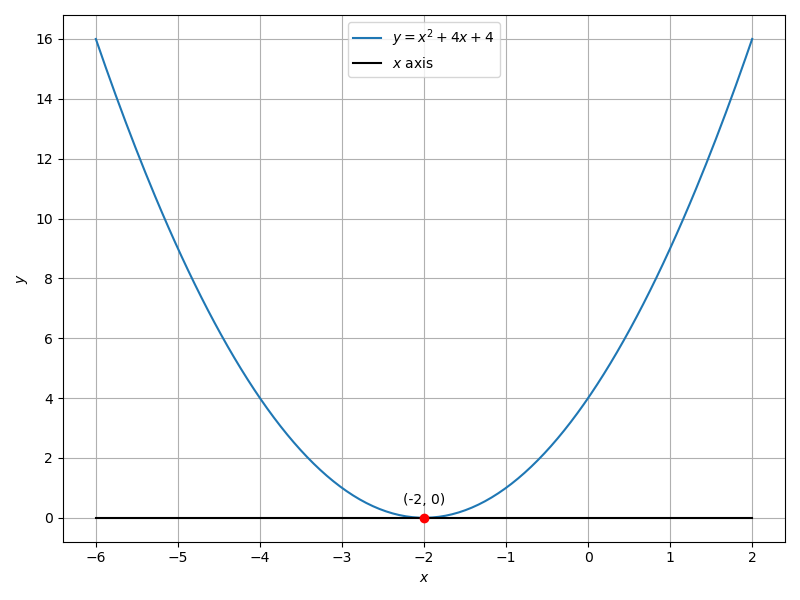
\includegraphics[width=0.75\linewidth]{figs/equal_roots.png}
    \caption{Parabola touching the $x$-axis at $x = -2$}
    \label{fig:EE26BTECH11229-14}
\end{figure}
\item 
A takes 6 days less than B to do a work. If both A and B working together can do it in 4 days, how many days will B take to finish it ?
\hfill (CBSE~2017)
\\
\solution
Let B take $x$ days to finish the work. Then A takes $x - 6$ days. From \eqref{eq:EE26BTECH11229-work},
\begin{align}
	\frac{1}{x} + \frac{1}{x-6} &= \frac{1}{4}
	\\
	\implies 4\brak{2x - 6} &= x\brak{x-6}
	\\
	\implies x^2 - 14x + 24 &= 0
\end{align}
From \eqref{eq:EE26BTECH11229-quad-formula},
\begin{align}
	x = \frac{14 \pm \sqrt{196 - 96}}{2} = \frac{14 \pm 10}{2} = 12 \text{ or } 2
\end{align}
For $x = 2$, A would take $-4$ days, which is not possible. Therefore, B takes $12$ days.
The following code verifies the solution
\begin{lstlisting}[frame=single, basicstyle=\rmfamily, escapeinside={(*@}{@*)}]
(*@\makebox[\dimexpr\linewidth-2\fboxsep-2\fboxrule\relax][c]{codes/work\_time.c}@*)
\end{lstlisting}
The following code generates \figref{fig:EE26BTECH11229-15}
\begin{lstlisting}[frame=single, basicstyle=\rmfamily, escapeinside={(*@}{@*)}]
(*@\makebox[\dimexpr\linewidth-2\fboxsep-2\fboxrule\relax][c]{codes/work\_time.py}@*)
\end{lstlisting}
\begin{figure}[H]
    \centering
    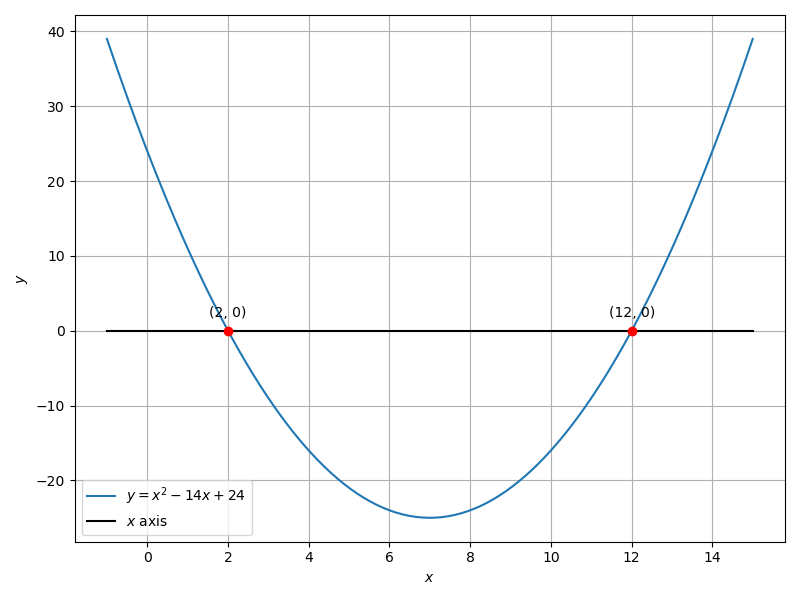
\includegraphics[width=0.75\linewidth]{figs/work_time.png}
    \caption{Work done by A and B}
    \label{fig:EE26BTECH11229-15}
\end{figure}
\item 
From the top of a tower, 100 m high, a man observes two cars on the opposite sides of the tower and in same straight line with its base, with angles of depression $30^{\circ}$ and $45^{\circ}$. Find the distance between the cars. \hfill [Take $\sqrt{3} = 1.732$]
\hfill (CBSE~2017)
\\
\solution
Let the foot of the tower be the origin, with the tower along the $y$-axis and the cars on the $x$-axis on opposite sides of the tower. Let the cars be at distances $d_1$ and $d_2$ from the foot, with angles of depression $45^{\circ}$ and $30^{\circ}$ respectively,
\begin{align}
	\vec{O} = \myvec{0 \\ 0}, \quad \vec{T} = \myvec{0 \\ 100}, \quad \vec{C}_1 = \myvec{d_1 \\ 0}, \quad \vec{C}_2 = \myvec{-d_2 \\ 0}
\end{align}
where $\vec{T}$ is the top of the tower. The vectors are
\begin{align}
	\vec{T}-\vec{C}_1 = \myvec{-d_1 \\ 100}, \quad \vec{O}-\vec{C}_1 = \myvec{-d_1 \\ 0}, \quad
	\vec{T}-\vec{C}_2 = \myvec{d_2 \\ 100}, \quad \vec{O}-\vec{C}_2 = \myvec{d_2 \\ 0}
\end{align}
From \eqref{eq:EE26BTECH11229-depression},
\begin{align}
	\cos 45^{\circ} &= \frac{\brak{\vec{T}-\vec{C}_1}^{\top}\brak{\vec{O}-\vec{C}_1}}{\norm{\vec{T}-\vec{C}_1}\norm{\vec{O}-\vec{C}_1}} = \frac{d_1}{\sqrt{d_1^2 + 10000}}
	\\
	\cos 30^{\circ} &= \frac{\brak{\vec{T}-\vec{C}_2}^{\top}\brak{\vec{O}-\vec{C}_2}}{\norm{\vec{T}-\vec{C}_2}\norm{\vec{O}-\vec{C}_2}} = \frac{d_2}{\sqrt{d_2^2 + 10000}}
\end{align}
Squaring both equations,
\begin{align}
	\frac{1}{2} &= \frac{d_1^2}{d_1^2 + 10000} \implies d_1^2 = 10000 \implies d_1 = 100 \text{ m}
	\\
	\frac{3}{4} &= \frac{d_2^2}{d_2^2 + 10000} \implies d_2^2 = 30000 \implies d_2 = 100\sqrt{3} \text{ m}
\end{align}
The distance between the cars is
\begin{align}
	\norm{\vec{C}_1 - \vec{C}_2} = \norm{\myvec{d_1 + d_2 \\ 0}} = d_1 + d_2 = 100\brak{1 + \sqrt{3}} = 100\brak{1 + 1.732} = 273.2 \text{ m}
\end{align}
The following code generates \figref{fig:EE26BTECH11229-8}
\begin{lstlisting}[frame=single, basicstyle=\rmfamily, escapeinside={(*@}{@*)}]
(*@\makebox[\dimexpr\linewidth-2\fboxsep-2\fboxrule\relax][c]{codes/tower\_cars.py}@*)
\end{lstlisting}
\begin{figure}[H]
    \centering
    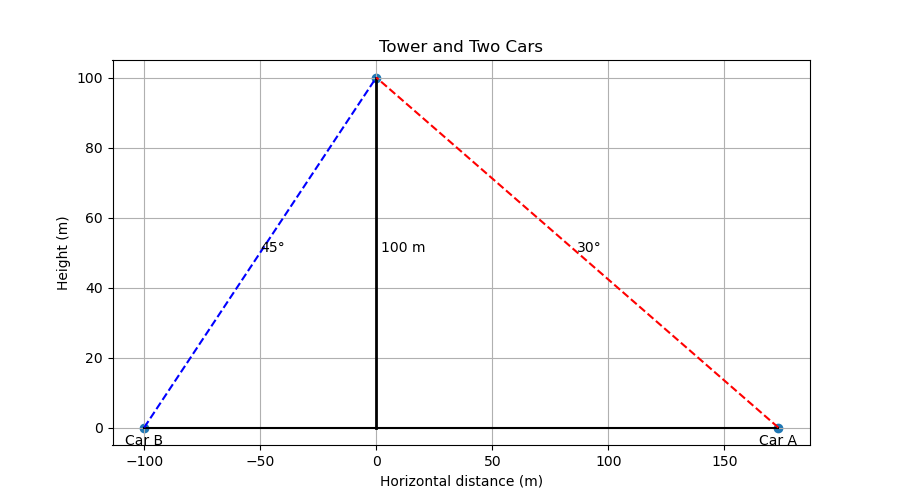
\includegraphics[width=0.75\linewidth]{figs/tower_cars.png}
    \caption{Tower and the two cars}
    \label{fig:EE26BTECH11229-8}
\end{figure}
\end{enumerate}
